\documentclass{standalone}
\usepackage{tikz}
\usetikzlibrary{patterns, positioning}
\usepackage[sfdefault]{ClearSans} %% option 'sfdefault' activates Clear Sans as the default text font
\usepackage[T1]{fontenc}

\begin{document}
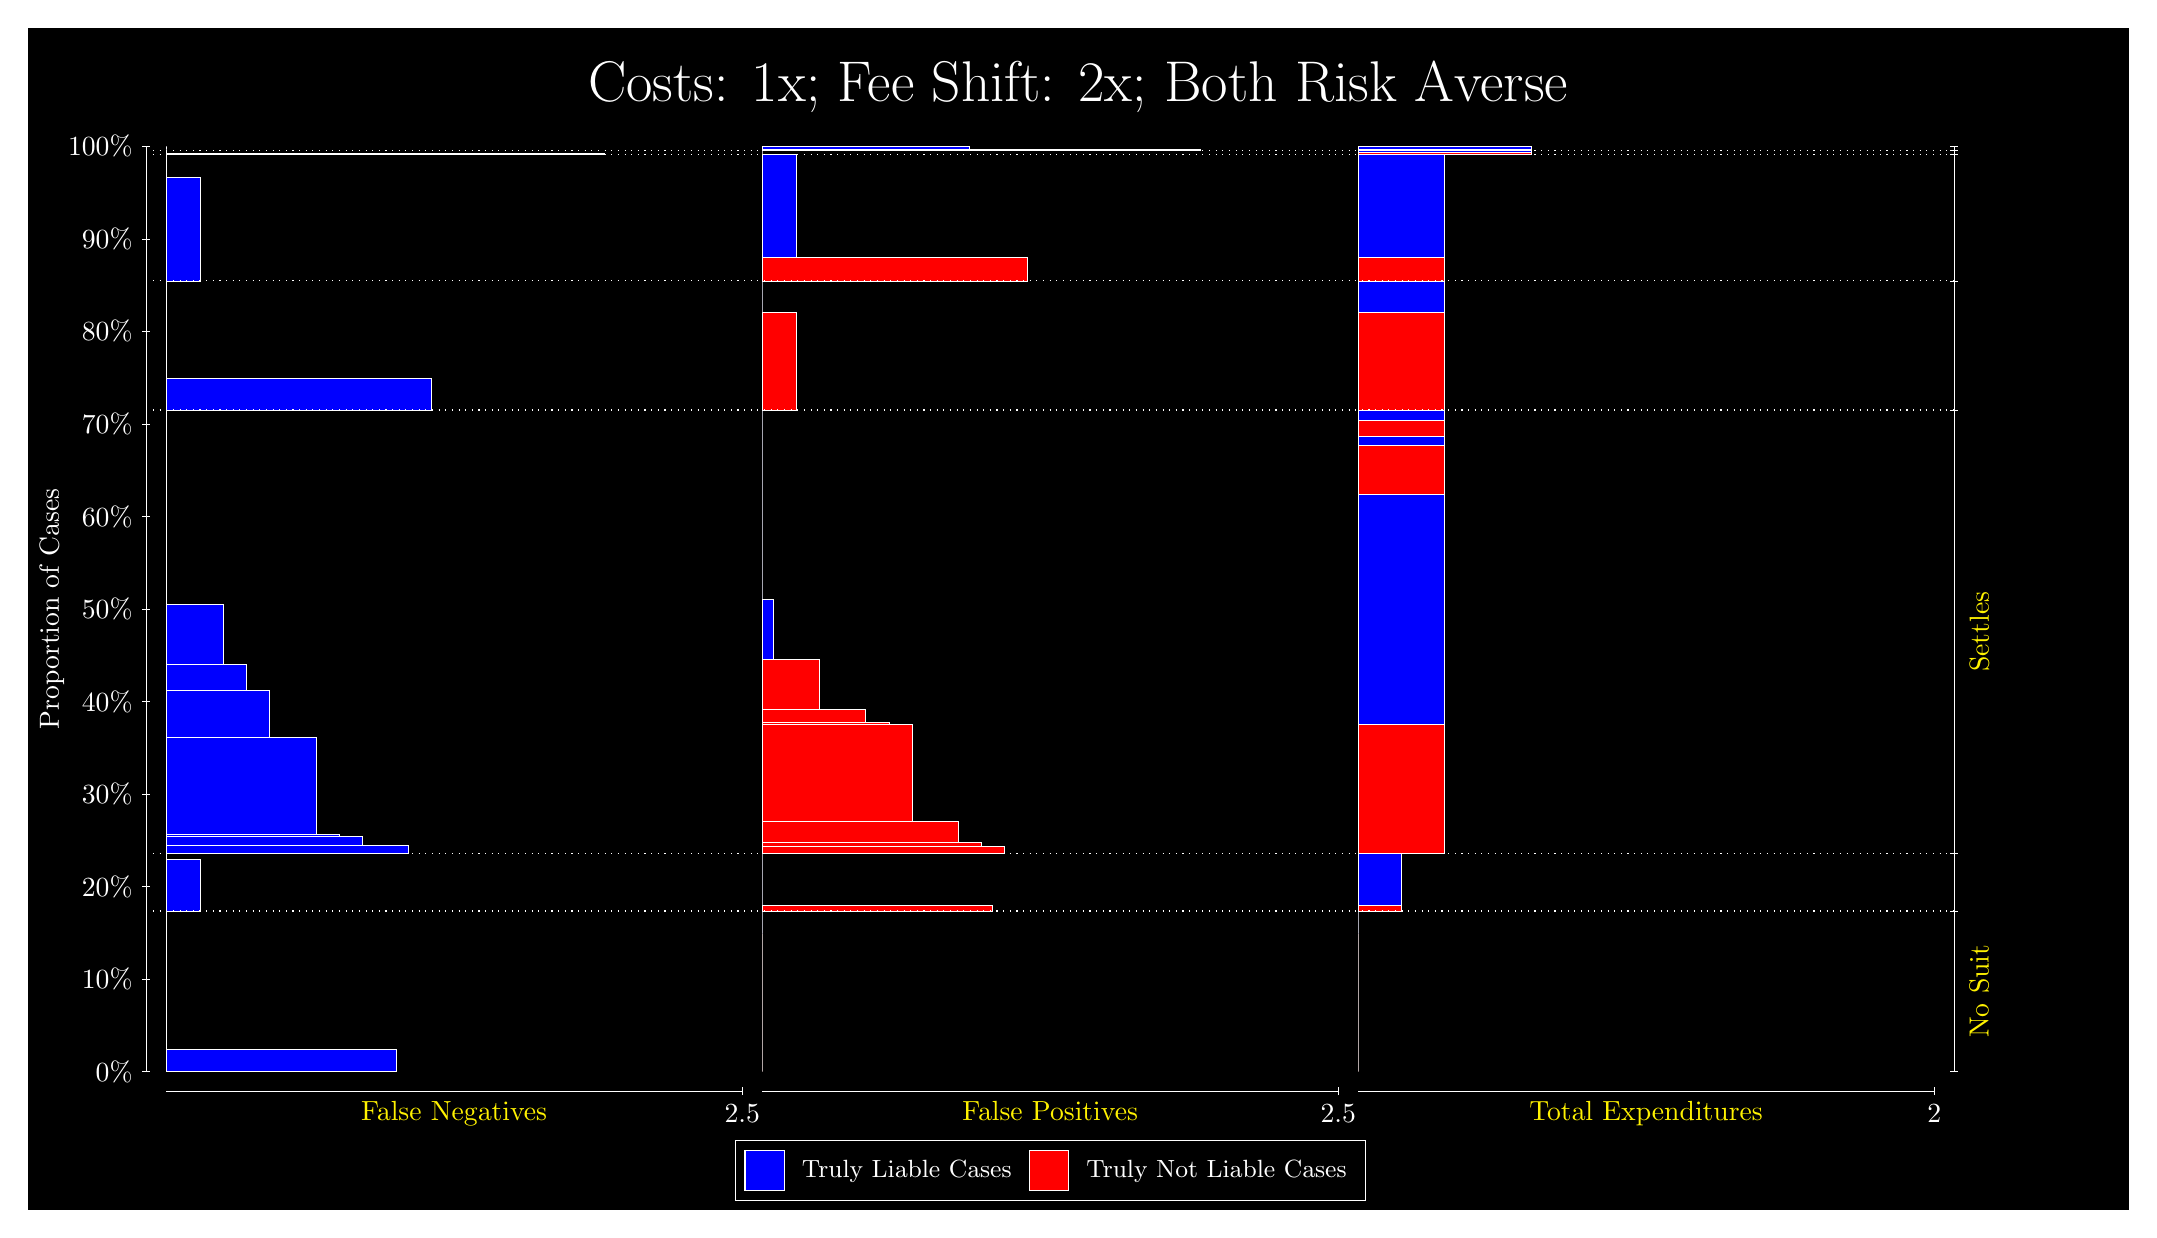
\begin{tikzpicture}
\draw[fill=black] (0,0) rectangle (26.667,15);
\draw[text=white] (0,13.5) rectangle (26.667,15) node[midway] {\huge Costs: 1x; Fee Shift: 2x; Both Risk Averse};
\draw[white, very thin] (1.5,1.75) -- (1.5,13.5);
\node[rotate=90, text=white, anchor=center] at (0.3, 7.625) {Proportion of Cases};
\draw[white, very thin] (1.45,1.75) -- (1.55,1.75);
\node[text=white, anchor=east] at (1.45, 1.75) {0\%};
\draw[white, very thin] (1.45,2.925) -- (1.55,2.925);
\node[text=white, anchor=east] at (1.45, 2.925) {10\%};
\draw[white, very thin] (1.45,4.1) -- (1.55,4.1);
\node[text=white, anchor=east] at (1.45, 4.1) {20\%};
\draw[white, very thin] (1.45,5.275) -- (1.55,5.275);
\node[text=white, anchor=east] at (1.45, 5.275) {30\%};
\draw[white, very thin] (1.45,6.45) -- (1.55,6.45);
\node[text=white, anchor=east] at (1.45, 6.45) {40\%};
\draw[white, very thin] (1.45,7.625) -- (1.55,7.625);
\node[text=white, anchor=east] at (1.45, 7.625) {50\%};
\draw[white, very thin] (1.45,8.8) -- (1.55,8.8);
\node[text=white, anchor=east] at (1.45, 8.8) {60\%};
\draw[white, very thin] (1.45,9.975) -- (1.55,9.975);
\node[text=white, anchor=east] at (1.45, 9.975) {70\%};
\draw[white, very thin] (1.45,11.15) -- (1.55,11.15);
\node[text=white, anchor=east] at (1.45, 11.15) {80\%};
\draw[white, very thin] (1.45,12.325) -- (1.55,12.325);
\node[text=white, anchor=east] at (1.45, 12.325) {90\%};
\draw[white, very thin] (1.45,13.5) -- (1.55,13.5);
\node[text=white, anchor=east] at (1.45, 13.5) {100\%};

\draw[white, very thin] (24.457,1.75) -- (24.457,13.5);
\draw[white, very thin] (24.407,1.75) -- (24.507,1.75);
\node[anchor=west] at (24.407, 1.75) {};
\draw[white, very thin] (24.407,3.7893) -- (24.507,3.7893);
\node[anchor=west] at (24.407, 3.7893) {};
\draw[white, very thin] (24.407,4.518) -- (24.507,4.518);
\node[anchor=west] at (24.407, 4.518) {};
\draw[white, very thin] (24.407,10.151) -- (24.507,10.151);
\node[anchor=west] at (24.407, 10.151) {};
\draw[white, very thin] (24.407,11.792) -- (24.507,11.792);
\node[anchor=west] at (24.407, 11.792) {};
\draw[white, very thin] (24.407,13.398) -- (24.507,13.398);
\node[anchor=west] at (24.407, 13.398) {};
\draw[white, very thin] (24.407,13.444) -- (24.507,13.444);
\node[anchor=west] at (24.407, 13.444) {};
\draw[white, very thin] (24.407,13.5) -- (24.507,13.5);
\node[anchor=west] at (24.407, 13.5) {};

\draw[white, very thin, fill=blue] (1.75,1.75) rectangle (4.6775,2.0376);
\draw[white, very thin, fill=red] (1.75,2.0376) rectangle (1.75,3.7893);
\draw[white, very thin, fill=blue] (1.75,3.7893) rectangle (2.1891,4.4413);
\draw[white, very thin, fill=red] (1.75,4.4413) rectangle (1.75,4.518);
\draw[white, very thin, fill=blue] (1.75,4.518) rectangle (4.8239,4.6252);
\draw[white, very thin, fill=blue] (1.75,4.6252) rectangle (4.2384,4.7438);
\draw[white, very thin, fill=blue] (1.75,4.7438) rectangle (3.9457,4.7617);
\draw[white, very thin, fill=blue] (1.75,4.7617) rectangle (3.6529,5.9903);
\draw[white, very thin, fill=blue] (1.75,5.9903) rectangle (3.0674,6.5913);
\draw[white, very thin, fill=blue] (1.75,6.5913) rectangle (2.7746,6.9174);
\draw[white, very thin, fill=blue] (1.75,6.9174) rectangle (2.4819,7.6846);
\draw[white, very thin, fill=red] (1.75,7.6846) rectangle (1.75,10.151);
\draw[white, very thin, fill=blue] (1.75,10.151) rectangle (5.1167,10.55);
\draw[white, very thin, fill=red] (1.75,10.55) rectangle (1.75,11.792);
\draw[white, very thin, fill=blue] (1.75,11.792) rectangle (2.1891,13.105);
\draw[white, very thin, fill=red] (1.75,13.105) rectangle (1.75,13.398);
\draw[white, very thin, fill=blue] (1.75,13.398) rectangle (7.3123,13.415);
\draw[white, very thin, fill=red] (1.75,13.415) rectangle (1.75,13.444);
\draw[white, very thin, fill=red] (1.75,13.444) rectangle (1.75,13.461);
\draw[white, very thin, fill=blue] (1.75,13.461) rectangle (1.75,13.5);
\draw[white, very thin, fill=red] (9.3189,1.75) rectangle (9.3189,3.5017);
\draw[white, very thin, fill=blue] (9.3189,3.5017) rectangle (9.3189,3.7893);
\draw[white, very thin, fill=red] (9.3189,3.7893) rectangle (12.246,3.866);
\draw[white, very thin, fill=blue] (9.3189,3.866) rectangle (9.3189,4.518);
\draw[white, very thin, fill=red] (9.3189,4.518) rectangle (12.393,4.612);
\draw[white, very thin, fill=red] (9.3189,4.612) rectangle (12.1,4.6565);
\draw[white, very thin, fill=red] (9.3189,4.6565) rectangle (11.807,4.9298);
\draw[white, very thin, fill=red] (9.3189,4.9298) rectangle (11.222,6.1552);
\draw[white, very thin, fill=red] (9.3189,6.1552) rectangle (10.929,6.1795);
\draw[white, very thin, fill=red] (9.3189,6.1795) rectangle (10.636,6.3557);
\draw[white, very thin, fill=red] (9.3189,6.3557) rectangle (10.051,6.9848);
\draw[white, very thin, fill=blue] (9.3189,6.9848) rectangle (9.4652,7.752);
\draw[white, very thin, fill=blue] (9.3189,7.752) rectangle (9.3189,10.151);
\draw[white, very thin, fill=red] (9.3189,10.151) rectangle (9.758,11.393);
\draw[white, very thin, fill=blue] (9.3189,11.393) rectangle (9.3189,11.792);
\draw[white, very thin, fill=red] (9.3189,11.792) rectangle (12.686,12.085);
\draw[white, very thin, fill=blue] (9.3189,12.085) rectangle (9.758,13.398);
\draw[white, very thin, fill=red] (9.3189,13.398) rectangle (9.3189,13.427);
\draw[white, very thin, fill=blue] (9.3189,13.427) rectangle (9.3189,13.444);
\draw[white, very thin, fill=red] (9.3189,13.444) rectangle (14.881,13.461);
\draw[white, very thin, fill=blue] (9.3189,13.461) rectangle (11.954,13.5);
\draw[white, very thin, fill=red] (16.888,1.75) rectangle (16.888,3.5017);
\draw[white, very thin, fill=blue] (16.888,3.5017) rectangle (16.888,3.7893);
\draw[white, very thin, fill=red] (16.888,3.7893) rectangle (17.437,3.866);
\draw[white, very thin, fill=blue] (16.888,3.866) rectangle (17.437,4.518);
\draw[white, very thin, fill=red] (16.888,4.518) rectangle (17.986,6.1552);
\draw[white, very thin, fill=blue] (16.888,6.1552) rectangle (17.986,9.0781);
\draw[white, very thin, fill=red] (16.888,9.0781) rectangle (17.986,9.7072);
\draw[white, very thin, fill=blue] (16.888,9.7072) rectangle (17.986,9.8144);
\draw[white, very thin, fill=red] (16.888,9.8144) rectangle (17.986,10.015);
\draw[white, very thin, fill=blue] (16.888,10.015) rectangle (17.986,10.151);
\draw[white, very thin, fill=red] (16.888,10.151) rectangle (17.986,11.393);
\draw[white, very thin, fill=blue] (16.888,11.393) rectangle (17.986,11.792);
\draw[white, very thin, fill=red] (16.888,11.792) rectangle (17.986,12.085);
\draw[white, very thin, fill=blue] (16.888,12.085) rectangle (17.986,13.398);
\draw[white, very thin, fill=red] (16.888,13.398) rectangle (19.083,13.427);
\draw[white, very thin, fill=blue] (16.888,13.427) rectangle (19.083,13.444);
\draw[white, very thin, fill=red] (16.888,13.444) rectangle (19.083,13.461);
\draw[white, very thin, fill=blue] (16.888,13.461) rectangle (19.083,13.5);
\draw[white, dotted] (1.5,3.7893) -- (24.457,3.7893);
\draw[white, dotted] (1.5,4.518) -- (24.457,4.518);
\draw[white, dotted] (1.5,10.151) -- (24.457,10.151);
\draw[white, dotted] (1.5,11.792) -- (24.457,11.792);
\draw[white, dotted] (1.5,13.398) -- (24.457,13.398);
\draw[white, dotted] (1.5,13.444) -- (24.457,13.444);
\draw[white, very thin] (1.75,1.5) -- (9.0689,1.5);
\node[text=yellow, anchor=north] at (5.4094, 1.5) {False Negatives};
\draw[white, very thin] (9.0689,1.45) -- (9.0689,1.55);
\node[text=white, anchor=north] at (9.0689, 1.45) {2.5};

\draw[white, very thin] (9.3189,1.5) -- (16.638,1.5);
\node[text=yellow, anchor=north] at (12.978, 1.5) {False Positives};
\draw[white, very thin] (16.638,1.45) -- (16.638,1.55);
\node[text=white, anchor=north] at (16.638, 1.45) {2.5};

\draw[white, very thin] (16.888,1.5) -- (24.207,1.5);
\node[text=yellow, anchor=north] at (20.547, 1.5) {Total Expenditures};
\draw[white, very thin] (24.207,1.45) -- (24.207,1.55);
\node[text=white, anchor=north] at (24.207, 1.45) {2};

\node[text=yellow, centered, rotate=90] at (24.777, 2.7696) {No Suit};

\node[text=yellow, centered, rotate=90] at (24.777, 7.3347) {Settles};





\draw (12.978300999999998,1.5) node[draw=none] (baseCoordinate) {};
\begin{scope}[align=center]
        \matrix[scale=0.5, draw=white, below=0.5cm of baseCoordinate, nodes={draw}, column sep=0.1cm]{
            \node[rectangle, draw, minimum width=0.5cm, minimum height=0.5cm, fill=blue] {}; &
            \node[draw=none, font=\small, text=white] (B) {Truly Liable Cases}; &
            \node[rectangle, draw, minimum width=0.5cm, minimum height=0.5cm, fill=red] {}; &
            \node[draw=none, font=\small, text=white] (B) {Truly Not Liable Cases}; \\
            };
\end{scope}

\end{tikzpicture}
\end{document}